

\documentclass{sig-alternate-05-2015}

% Include useful packages
\usepackage{graphicx}
\graphicspath{ {images/} }
\usepackage{float}


\begin{document}

% Copyright
\setcopyright{acmcopyright}

\title{Approaches to Incorporating Whole Genome Information in the context of Clincal Prediction}

\author{
% You can go ahead and credit any number of authors here,
% e.g. one 'row of three' or two rows (consisting of one row of three
% and a second row of one, two or three).
%
% The command \alignauthor (no curly braces needed) should
% precede each author name, affiliation/snail-mail address and
% e-mail address. Additionally, tag each line of
% affiliation/address with \affaddr, and tag the
% e-mail address with \email.
%
% 1st. author
Siddharth Avadhanam\\
       \email{avadhana@msu.edu}
}
% There's nothing stopping you putting the seventh, eighth, etc.
% author on the opening page (as the 'third row') but we ask,
% for aesthetic reasons that you place these 'additional authors'
% in the \additional authors block, viz.
\date{\today}
% Just remember to make sure that the TOTAL number of authors
% is the number that will appear on the first page PLUS the
% number that will appear in the \additionalauthors section.

\maketitle



\section{Problem Description}

The high-dimensionality and complexity of data coming in from Genome Wide Association Studies
poses a whole range of statistical and computational challenges in finding genetic covariates of important phenotypes
( disease, yield , height etc). These data commonly contain thousands of individuals with information on
hundreds of thousands of markers. \cite{zhang_chapter_2012}

An important issue which has been given considerable attention in the statistical genetics
literature is how to choose a subset of these markers so that the analysis of these data with standard commodity hardware and statistical methods
becomes more tractable.\cite{de_los_campos_whole-genome_2013} Methods which analyze a single-marker at a time are popular, but are severly limited in that they do not take into account
interactions between markers, and come with their own set of challenges related to multiple testing.\cite{moskvina_multiple-testing_2008}

It is thus becoming increasingly important to explore methods that incorporate information from
the whole genome and possibly from outside the domain of traditional statistics.

Methods that incorporate information form the whole genome simultaneously are finding increasing success.
These apporaches as a whole are better suited toward tackling the problems of missing heritability and are able to explain a much better
proportion of the variation for multifactorial outcomes such as height.\cite{eichler_missing_2010}
The complexity of the underlying biology demands approaches that can incorporate information from across the genome and possibly use multiple sources of genetic information.

These problems form the primary motivation for this work. Specifically, we look at how machine learning methods can help us consider all the genetic marker information simultaneously.
Vairable shrinkage and selection methods such as the Lasso and the Elastic Net have been applied to these types of high-dimensional problems with considerable success.\cite{waldmann_evaluation_2013} Here we will focus particularly on the
Elastic Net. We will also be considering Kernel based approaches and how they can be applied to genomic enabled clinical prediction.
Kernel methods have immense flexibility ( can be adopted towards multiple data-types ) and are particularly useful for high-dimensional problems.\cite{wang_kernel_2015}

Another angle we will take toward tackling this problem is the use of Bayesian methodology. Bayesian approaches are increasingly being used in the domain
of statistical genetics due to the rapidly declining costs of computing resources, and advances in
techniques for approximating high-dimensional integrals (such as the Markov Chain Monte Carlo).

Also notably, Bayesian methods obviate the need for cross validation due to the ability to estimate hyper-parameters guided by the data alone.
These appraoches are also more intuitive, and are generative models that allow us to sample parameters
form the posterior distributions. However, our primary reason in using these approaches is the ability to incorporate simultaneous shrinkage and selection through the
use of an appropriate prior (BayesB or BayesC), and to exploit priors that incorporate size-of-effect dependent shrinkage. We will see that these methods give us
strikingly good cross-validation results.

In this work I propose to evaluate bayesian methodology and contrast it with classical approaches in the context of genomic-enabled prediction. The objective here will be two fold.
Firstly, We will evaluate methods to incorporate information from the entire genome simulataneously ( the so called whole-genome approach ) as opposed to one marker at a time.
Second, we will look evaluate these methods through a simulation by studying various genetic-trait architecutres.
We will see how some methods better explain the phenotypic variance, as well as give us more accurate estimates. Classical whole genome regression
approaches we look at include methods such as ridge-regression and the Elastic Net.\cite{waldmann_evaluation_2013}

All methods will be implemented in R. Bayesian methods will be executed using the BGLR (Bayesian Generalized Linear Regression) package by Perez et al.\cite{perez_genome-wide_2014} which provides a powerful modelling framework for incorporating bayesian regressions.
Differential shrinkage and marker selection can be implemented with an adequate choice of prior provided as options in the package, as well as the ability to include single or multi-kernel methods.

A good example of the motivation behind this work can be found in de los Campos et al. \cite{de_los_campos_predicting_2010} I will implement some of the more succesful approaches in a
an example mice dataset provided by the Wellcome Trust and that can be found online freely. The simulations will be carried out using the same data.

\begin{figure}
  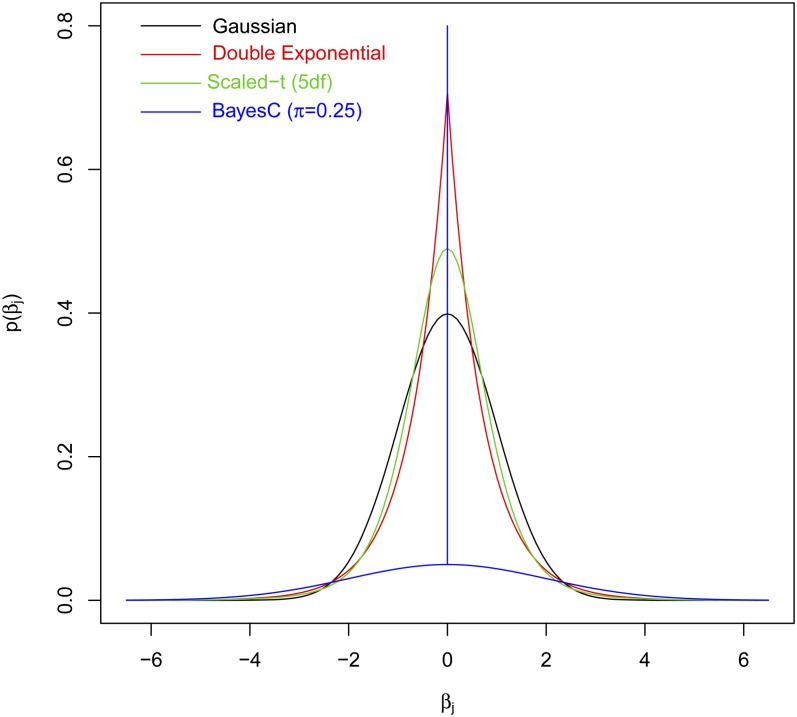
\includegraphics[width=8cm]{./Images/BGLR.jpg}
  \centering
  \caption{Figure \ref{fig:BGLR} by Perez et al.\cite{perez_genome-wide_2014} shows different prior densities implemented in BGLR}
  \label{fig:BGLR}
\end{figure}

\begin{figure}
  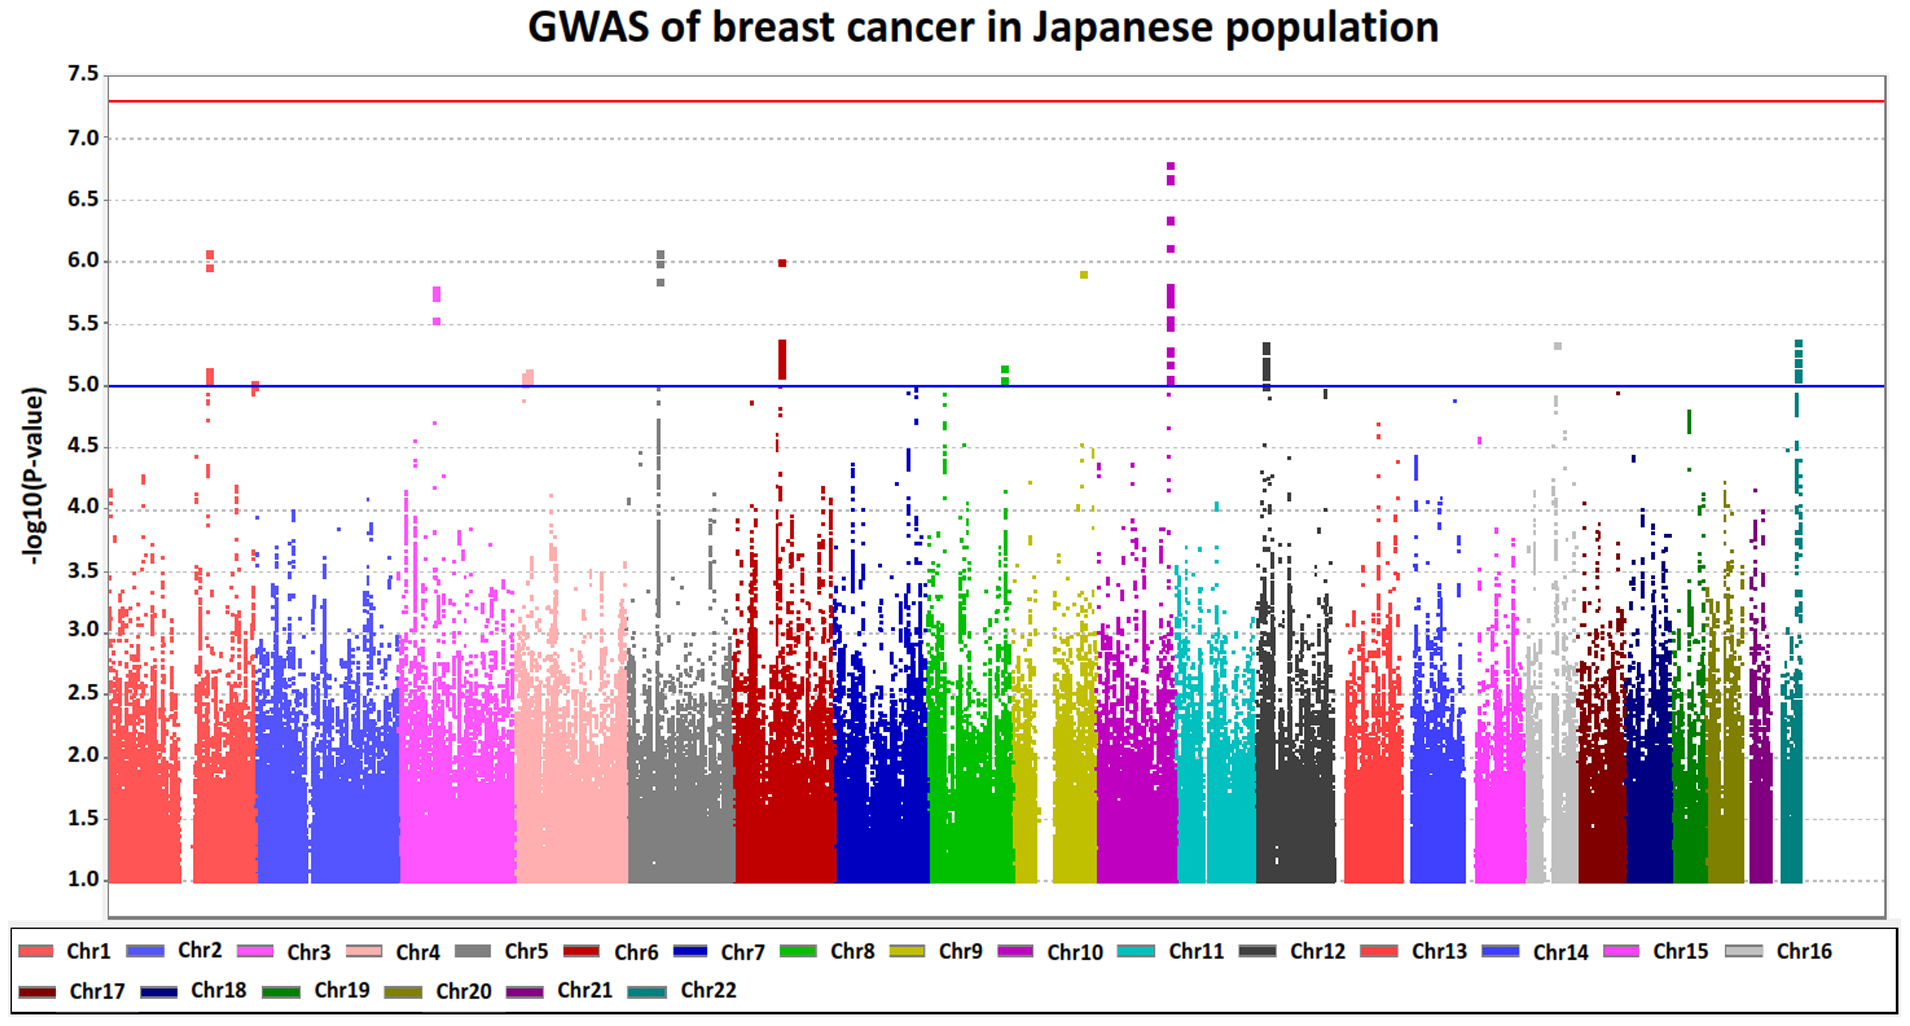
\includegraphics[width=8cm]{./Images/manhattan_plot.png}
  \centering
  \caption{Figure \ref{fig:manhattan1} shows an example manhattan plot by Low et al.\cite{low_genome-wide_2013} constructed from single marker regression across the genome. The y-axis is
  the $ -log(pvalue) $ and the x-axis contains SNP positions colored by chromosome.}
  \label{fig:manhattan1}
\end{figure}


\section{Related Work}

There is considerable literature in statistical learning approaches towards the analysis of GWAS data. Earlier work has
touched upon single marker regression methods and the whole host of approaches that can be applied to
deal with the multiple-testing issues.

Penalized regression methods such as ridge regression,\cite{austin_penalized_2013}
variable selection methods such as the lasso  and dimensionality reducing approaches such as principal components \cite{price_principal_2006} have all been applied and studied extensively in the analysis of
genome-wide data.

Bayesian methods are seeing a resurgence in many fields apart from genetics, and there are many recent works that dwelve into their application
to genetics in detail. There is a good understanding on the impact of genetic architecture, including marker density, span of linkage disequilibrium
and number of causal QTLs on the performance of Bayesian methods. This is also something we explore in this work.

The discovery of gene-gene interactions is an active area of research where machine learning tools are being extensively employed \cite{upstill-goddard_machine_2013}
Bayesian methods and mixed models approaches within specific communities such as animal breeding have been
studied and applied for a long time, and are increasingly being used with genome-wide data. \cite{de_los_campos_whole-genome_2013}.

The issue of missing heritability and multi-factorial traits have gotten considerable attention in the literature. Multi-omics approaches toward improving prediction accuracy
are starting to gain traction with increase in the availability of computational resources. In addition to better prediction, these approaches can be particularly illuminating when
it comes to the biological mechanisms being studied. \cite{kim_multi-omics_2016}
An example would be to try and understand how much of the variation in the trait of interest can be explained by epigenetic variation, and is one of the things we are interested in here.

Another direction in the literature makes use of the methods mentioned so far to better understand the pathogenetic etiology of disease by studying genetic overlap between the disease and it's comorbidites.

\section{Data Description}

The Dataset is a mice dataset with 1814 observations and 10,346 SNPs from the Wellcome Trust and is freely available online
There are about as many male mice as there are female mice. BMI's have been adjusted relative to an average and that is why we have negative
values in the Data.

We center and scale the data before and compute $XX'$ to get a Relationship matrix which we use for our kernel model.
The marker matrix has been preprocessed and Quality controlled. Markers with minor allele frequency less than 0.05 have been removed and the rest have been tested for Hardy Weinberg Equilibrium.

The phenotype matrix contains data on obesity. Our primary outcome of interest will be BMI, which we try to predict.
Cage Density, Litter size, and sex are also important covariate to control for. The Cage number has also been added to the model as a random effect.


\section{Methods and Results}

This section is broken up into two parts. The first part of the study is a comparative analysis of various models applied to the mice dataset.
The second part is a simulation study that focuses on evaluating a few of the more promising approaches across different genetic trait architectures.

\subsection{Part I : Comparative Analysis}

As a first step towards model fitting and comparison, we evaluate the performance of the Elastic Net model at different values of the mixing parameter.
The Elastic Net is a regularized regression method that
linearly combines the L1 and L2 penalties of the lasso and ridge methods.\cite{_elastic_2017}
The cross-validation prediction accuracy is plotted against the value of alpha, and is shown below (Figure 3).  Here, we evaluate the optimal lambda based on cross-validation
for each value of alpha.

The results seem to indicate that a low value of the mixing parameter give very poor results. Upon incorporating some amount of variable selection, the model gets
drastically better, with only modest gains upon increasing alpha further. This model gives the best performance in the limit of the Lasso Model.
(Figure 3)

\begin{figure}
  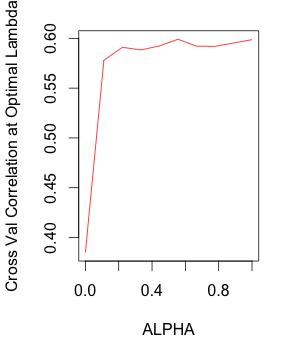
\includegraphics[width=8cm]{./Images/elasticnet.png}
  \centering
  \caption{Figure \ref{fig:elasticnet} shows the results of our Elastic Net model evaluated across different values of alpha.}
  \label{fig:elasticnet}
\end{figure}


This leads us to suspect that a combination of selection and shrinkage might work much better for high-dimensional genetic inference, and forms the most salient theme for
the rest of this discussion.

Next, we evaluate a kernel model using the Reproducible Kernel Hilbert Spaces model implemented in the R package BGLR.
We will compute a Gaussian kernel form the marker matrix, and fit a Gaussian process model.The implementation of Gaussian processes in BGLR exploits
the equivalence between these processes and random regressions on principal components \cite{perez_genome-wide_2014}

We see the that the RKHS model incorporates genetic information pretty well and gets us a prediction accuracy of 0.56.
We get nice mixing with the Error variance, and a heritability estimate of about 0.18. Inference is pretty robust, 0.51 of the variance in the phenotype is left unexplained by our model.
An advantage of this approach is that it uses all the information contained in the markers data. It also gives good performance while being omputationally less expensive.
This kind of model also has the unique advantage of interpretability in certain situations. It can, for example, be interpreted better to shed light on how much genetics actually contributes to a
certain condition or disease. It would be particularly useful when dealing with multi-factorial traits.

We can visualize the performance of this model by extracting the trace plots of the MCMC sampler. These plots gives us insight not only into the
inferential quality of the method via trace plots of the error variance and the genetic variance (Figures 4 and 5) , but also the performance of the models
via a correlation plot (Figure 6)

\begin{figure}
  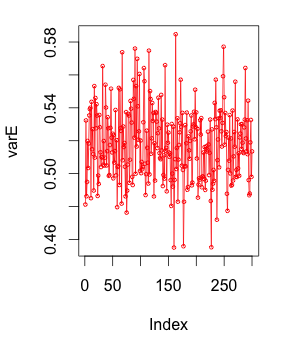
\includegraphics[width=8cm]{./Images/kernelplot_varE.png}
  \centering
  \caption{Figure \ref{fig:kernelvarE} shows a trace plot of the error variance from the MCMC sampler.
  We can see that the mixing is pretty good, and the inference is robust . }
  \label{fig:kernelvarE}
\end{figure}

\begin{figure}
  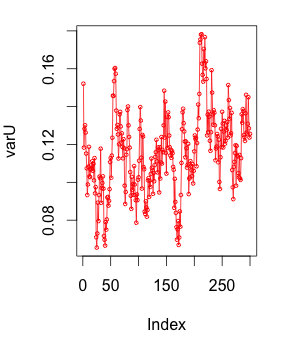
\includegraphics[width=8cm]{./Images/kernelplot_varU.png}
  \centering
  \caption{Figure \ref{fig:kernelvarU} shows a trace plot of the variance attributed to the random effect associated with levels of the
  Kernel Matrix. The mixing is not as good as the error variance, as there is lesser information to infer this parameter. The inference is still
  pretty robust and we get a stable heritability estimate.}
  \label{fig:kernelvarU}
\end{figure}

\begin{figure}
  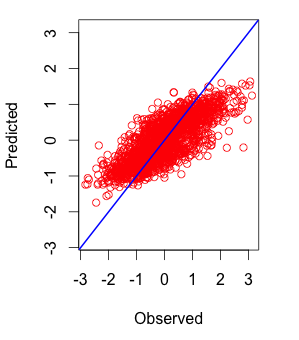
\includegraphics[width=8cm]{./Images/Kernelmodel_1.png}
  \centering
  \caption{Figure \ref{fig:corrplot} shows the correlation between predicted and observed values of the target variable.}
  \label{fig:corrplot}
\end{figure}



One obvious shortcoming of this approach is that it cannot infer causative markers, as we collapse that information into a covaraince matrix. As we shall see, while performing reasonably, it is limited with respect to the potential
gains in prediction accuracy using all the marker information.

Next, we look at Bayesian methods for dealing with the high-dimensional marker information directly. All the method that I go into below use different priors which
enable us to carry out parameter shrinkage, selection, or some combination of both ( much like the elastic net with its mixture of penalties.)
We look at estimation using Bayes Ridge Regression, which uses a Gaussian prior and is identical to its non-Bayesian counterpart.
The Gaussian prior is centered about zero, and it can be shown theoretically that this produces shrinkage identical to using ridge regression.
Intuitively, incorporating the a-priori belief that the parameters have a higher
probability of being close to zero using a Gaussian prior is identical to enforcing that requirement using a regularized square-loss function and
penalizing ${ \lVert \beta^2 \rVert }$ .\cite{perez_genome-wide_2014}

We also evaluate the Bayes Lasso which uses a double exponential prior, the BayesA, which uses a scaled-t prior, and the BayesB which uses a
prior that is finite-mixture denisty of a point mass at zero and a scaled-t slab. (Figure 2)
Note that the BayesB is the only prior that incorporates selection as there is non-zero probability that beta is assigned an effect of size zero. Also,
it is important to note that the Bayes Lasso and Bayes A approaches incorporate size-of-effect dependent shrinkage. This can be understood by contrast it
with the Double-Exponential prior of the Bayes Lasso and the scaled-t prior of the Bayes A with the normal prior of the Bayes Ridge Regression. A normal prior
causes uniform shrinkage just like it's frequentist counterpart, but using the scaled-t or double exponential priors induces size-of-effect dependent shrinkage. \cite{perez_genome-wide_2014}

A few trace plots that give insight into the model performance as it runs are supplied. They are provided earlier for the RKHS model and below for the Bayes Lasso Model (Figure 7).
We also visualize the actual phenotypic values versus the predicted genomic values for the Bayes Lasso (Figure 8)
These plots for the Bayes Lasso are typical, and plots for BRR, BayesA and BayesB look similar.

\begin{figure}
  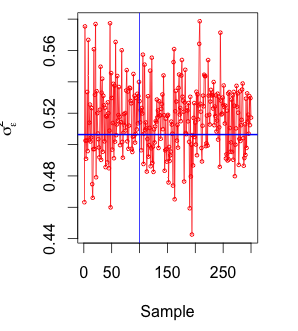
\includegraphics[width=8cm]{./Images/BLvarE.png}
  \centering
  \caption{Figure \ref{fig:BLvarE} Trace plot of the error variance for the Bayes Lasso model. We see that the mixing is not as good as for the
  Kernel model}
  \label{fig:BLvarE}
\end{figure}

\begin{figure}
  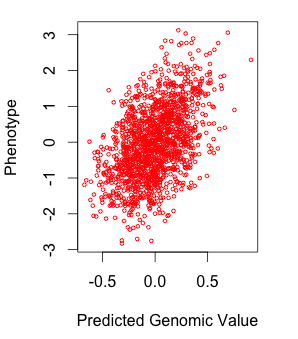
\includegraphics[width=8cm]{./Images/BLplot1.png}
  \centering
  \caption{Figure \ref{fig:corrgen} shows the correlation between predicted and observed values of the target variable.}
  \label{fig:corrgen}
\end{figure}

It can be seen from the trace plot of the MCMC sampler for the error variance (Figure 7) that the mixing for the Bayes Lasso Model is not as good as for the
Kernel model. This is to be expected as we do not use all the information available in the genotypes for inference here. The mixing will be better
for the BayesA and BayesB models.

Overall, the comparative performance of these models can be seen in the table provided below.

\begin{table}[h!]
\centering
 \begin{tabular}{||c c c c c||}
 \hline
 ModelName & Accuracy & Time	& Fit	& VarE\% \\
 \hline
  RKHS & 57\%	& 122	& 3507	& 51\% \\
 \hline
 BRR & 50.3\%	& 210	& 3490	& 50.1\% \\
 \hline
 BL	& 58\%	& 210	& 3517	& 50.6\% \\
 \hline
 BA	& 60.5\%	& 218 & 3504 & 50.7\% \\
 \hline
 BB	& 79.2\%	& 226	& 3539 & 52.4\% \\
 \hline
 EN	& 50.5\%	& 805 &	NA	& 49.9\% \\
 \hline
\end{tabular}
\caption{Table of Model Performace}
\label{table:1}
\end{table}

Here we see that the Bayes Ridge Rigression and the Elastic Net (for optimal alpha ) perform relatively poorly
compared to the other Bayesian approaches. Furtherm the Elastic Net takes a large amount of time to compute, however this may be due to implementational
details. Our RKHS model performs relatively quickly, however, the computation of the kernel matrix may be limiting as the size of the marker dataset increases.

The Bayes Lasso and BayesA model perform comparably, and better than the RKHS, ELastic Net and Ridge Regression approaches. As mentioned before,
these priors incorporate differential shrinkage of parameter estimates based on size-of-effect, and this may be the reason why we see better performance.
For simple trait architectures, it would seem that incorporating these priors for shrinkage gives us much better statistical power to capture the true signals.

Finally, The BayesB shows strikingly improved performance over the rest.
This is the onnly approach considered that incorporates a finite-mixture prior ( point mass at zero and
scaled t-slab) and hence simulatenously selects and shrinks parameter estimates.
These differences between the Bayes Ridge Regression, Bayes Lasso, BayesA and BayesB models will be made more clear
by observing the plots provided in the simulation study section.

In conclusion,
if our purpose is not to select significant SNPs, Kernel approaches are faster and more robust for inferring genetic contribution to a phenotype, or
for prediction. As we will see in the next section, these methods also work well across genetic trait architectures.

In the Elastic Net we see how incorporating some amount of variable selection is much better for inference, and in particular works best for Elastic Net with some
value of the mixing parameter around 0.5-0.6. Improvements over this are modest and are attributable to sampling error.
But we also see how slow this method is to compute and that it fares considerably worse at cross-validation prediction accuracy compared to some
of the other methods.

The Bayesian Lasso and BayesA, which use a Double exponential prior and Scaled-t prior respectively perform much better than the previous methods.
These methods are notably different from Frequentist approaches in that they allow us to incorporate size-of-effect dependent variable shrinkage with priors that are more
sharply peaked around zero.

The most promising method is the BayesB. It outperforms all the other approaches and seems to suggest, corroborating our result with the Elatic Net, that
incorporating a mixture of shrinkage and selection is the most promising general approach. BayesB method uses a mixture of a point mass at zero
and a scaled-t slab which allows for variable selection as there is a non-zero probability that the effect will be assigned a zero value.


\subsection{Part II : Simulation Study}

For the second part of our study, we conducted a simulation study to test these methods accross a variety of trait architecture.
To acheive this, we simulated phenotypes with 10,20,50 and 100 causative markers ( called QTLs ) and fixed heritability = 0.5
and evaluated cross validation performance across these architectures for the Bayes Ridge Regression, Bayes Lasso, BayesA and BayesB.

We can visualize the difference in the results by graphing the ground truth QTLs and those selected by all our models. These plots have been
made for the case of 20 simulated true QTLs. Figure \ref{fig:sim2_1}  shows the results for ground truth (Blue points), Bayes Lasso inference (Black),
and BayesA inference (Red). Figure \ref{fig:sim2_2} shows BRR inference in green, with BayesA performance removed for ease of inspection.

\begin{figure}
  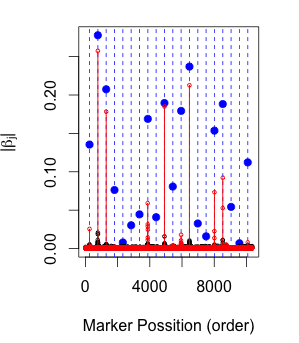
\includegraphics[width=8cm]{./Images/sim2_1.png}
  \centering
  \caption{Shows the true signal and estimated signal for marker effects across models}
  \label{fig:sim2_1}
\end{figure}

\begin{figure}
  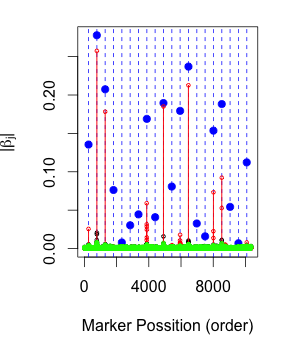
\includegraphics[width=8cm]{./Images/sim2_2.png}
  \centering
  \caption{ Shows the true signal and estimated signal for marker effects across models}
  \label{fig:sim2_2}
\end{figure}

It can be seen that the Bayes Lasso and Bayes A method both perform selection equally well, while the BayesA method has the added advantage of
doing much better at estimating the strength of the effect. The Bayes Ridge Regression signal has a lot of noise, and a few peaks at the true effects.
Overall, it's performance is very poor.

The Results suggest that incorporating simultaneous shrinkage and selection by using an appropriate prior
is a powerful method for prediction or causal inference across architectures. Figure \ref{fig:simfinal} shows the results for the performance of the models across
architectures.


\begin{figure}
  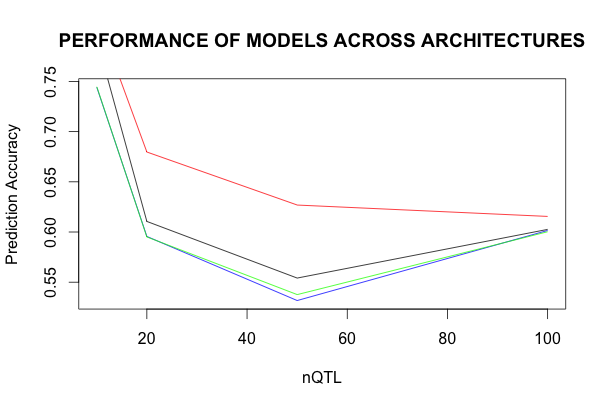
\includegraphics[width=8cm]{./Images/simplot_final.png}
  \centering
  \caption{ Results for the performance of the models across architectures.}
  \label{fig:simfinal}
\end{figure}


We see that as we increase the number of markers contributing to the trait, the performance of these models converges. This is to be expected, and
we can conlude that the value of using the Bayesian approach with a finite mixture prior is greatest for traits controlled by a few genes. Surpringly, the
performance of the Bayes Lasso, Bayes Ridge Regression and the Kernel Model seem to improve for a more dense trait architecture.

\section{Discussion}

We have seen that certain priors vastly outperform other methods. It seems that those that are sharply peaked around zero share
favourable characteristics. A future direction for this work is understanding in more detail why this is the case.

A major result from this study is that a combination of selection and shrinkage in a Bayesian cotext works well across trait architectures. This may be because of the unique nature of
genetic causation. We usually have a handful of genes scattered across the genome that contribute towards a trait, even for multi-factorial traits. Such methods may be well poised
to detect a signal in the case of high-dimensional data with sparse signals.

Another major result from the simulation section of this study is the convergence of model performance with different genetic architecutures. We can
see that these methods have the most merit for diseases that may have a few genetic factors responsible for it. A lot of nuerodegenerative diseases as
well as cancers share this feature, and the BayesB approach is very promising to approach these problems.

We haven't explored changing the heritability and span of LD for the genetic traits, and these are very important considerations.
Further, the example dataset and the simulations we used may be somewhat unrealistic or naive. These methods need to be explored in more detail
for more complex data and simulation conditions.

Another important limitation is that the Elastic Net approach may be slower due to implementational details, and those results should be treated with
caution.

\bibliography{cse_847_final}
\bibliographystyle{unsrt}
\end{document}
